\begin{pastexam}[label={px:df3-111-ds-02}]{地方三等資訊處理 111 年 第二題}
（申論；20 分）

常用的算術運算式（Arithmetic Expression）有：中序運算式（Infix Expression）、前序運算式（Prefix Expression）、
後序運算式（Postfix Expression）三種表示法，考慮下面的算術運算式（Arithmetic Expression）並回答下列問題：
\[
((6 \times (5 - 3)) - (1 + 2)) \times (((4 + 2) / 3) + (5 \times 4))
\]
\begin{itemize}[leftmargin=2.2em, nosep]
\item[㈠] 請寫出其前序運算式（Prefix Expression）。（5 分）
\item[㈡] 請繪出其算術運算樹（Expression Tree）。（5 分）
\item[㈢] 請說明如何以此算術運算樹計算出算術運算式的值，並一步一步列出運算過程。（10 分）
\end{itemize}
\end{pastexam}

\begin{pastsoln}
答案：㈠ $\times\ -\ \times\ 6\ -\ 5\ 3\ +\ 1\ 2\ +\ /\ +\ 4\ 2\ 3\ \times\ 5\ 4$。 ㈡ 樹畫在下面。 ㈢ 用後序走訪由下而上
計算，值是 $198$。

\textbf{㈡ 運算樹}（資結書第~7.7~節）：括號已經完全標出每個運算的範圍，最外層是中間那個 $\times$，它是根；左運算元
$(6 \times (5-3)) - (1+2)$、右運算元 $((4+2)/3) + (5 \times 4)$ 再各自往下拆。 運算子是內部節點，數字是葉子。
\begin{center}
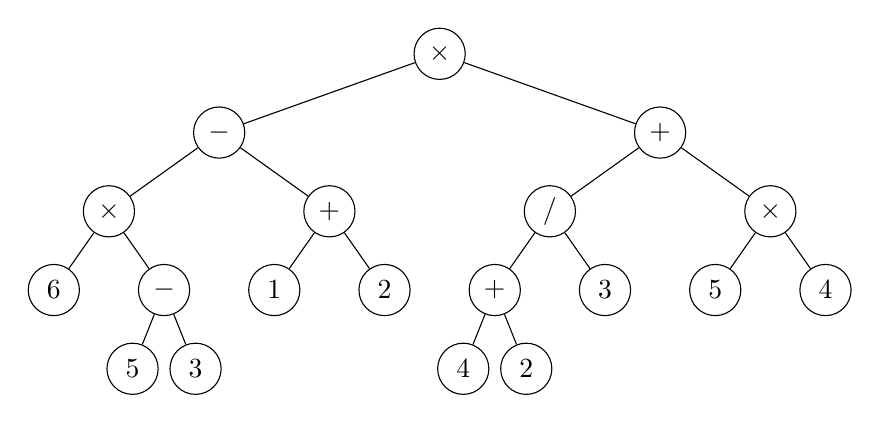
\begin{tikzpicture}[every node/.style={circle,draw,minimum size=6.5mm,inner sep=0pt},
  level distance=10mm, level 1/.style={sibling distance=56mm}, level 2/.style={sibling distance=28mm},
  level 3/.style={sibling distance=14mm}, level 4/.style={sibling distance=8mm}]
\node {$\times$}
  child {node {$-$}
    child {node {$\times$} child {node {6}} child {node {$-$} child {node {5}} child {node {3}}}}
    child {node {$+$} child {node {1}} child {node {2}}}}
  child {node {$+$}
    child {node {$/$} child {node {$+$} child {node {4}} child {node {2}}} child {node {3}}}
    child {node {$\times$} child {node {5}} child {node {4}}}};
\end{tikzpicture}
\end{center}

\textbf{㈠ 前序運算式}：對運算樹做前序走訪（根、左、右）。 左子樹的前序是 $-\ \times\ 6\ -\ 5\ 3\ +\ 1\ 2$，右子樹是
$+\ /\ +\ 4\ 2\ 3\ \times\ 5\ 4$，所以
\[
\times\ -\ \times\ 6\ -\ 5\ 3\ +\ 1\ 2\ +\ /\ +\ 4\ 2\ 3\ \times\ 5\ 4.
\]
（後序是 $6\ 5\ 3\ -\ \times\ 1\ 2\ +\ -\ 4\ 2\ +\ 3\ /\ 5\ 4\ \times\ +\ \times$。）

\textbf{㈢ 計算方法。} 一個運算子節點的值，要等它的兩棵子樹的值都算好才能算，所以用\textbf{後序走訪}：先遞迴算出
左子樹的值、再算右子樹的值，最後把節點的運算子套在兩個值上；葉子的值就是它的數字。 寫成遞迴：
\[
\mathit{eval}(x) = \begin{cases} x \text{ 的數字}, & x \text{ 是葉子}, \\
\mathit{eval}(x.\mathit{left})\ \mathit{op}(x)\ \mathit{eval}(x.\mathit{right}), & \text{其他}. \end{cases}
\]
照後序的順序，依次算出的節點是：
\begin{enumerate}
\item $5 - 3 = 2$
\item $6 \times 2 = 12$
\item $1 + 2 = 3$
\item $12 - 3 = 9$（根的左子樹算完）
\item $4 + 2 = 6$
\item $6 / 3 = 2$
\item $5 \times 4 = 20$
\item $2 + 20 = 22$（根的右子樹算完）
\item $9 \times 22 = 198$（根）
\end{enumerate}
所以運算式的值是 $198$。 等價的做法是用堆疊計算後序運算式（資結書第~6.3~節）：讀到數字就推入，讀到運算子就
彈出兩個數運算再推回，運算的順序和上面九步完全相同。
\end{pastsoln}
